\chapter{Approach}
\label{ch:approach}

\section{Proposed Solution}
As has been discussed in chapter \ref{ch:related}, there is a need for a tool to detect as much as possible syntax errors in RDF documents. As a result to this need, this study was held and this chapter will cover the approach used in the proposed solution.

	\vspace{5mm} %5mm vertical space

 To represent the approach in more clear way, {\it figure \ref{Fig:Approach}} was invented. It shows the technique used to handle an RDF text, having some syntax errors. follows are the sequence steps which highlight the main milestones of this approach:
 \begin{enumerate}[label=(\alph*)]
\item \textbf{Reading RDF text}: a ordinary RDF file is submitted to our application. The application starts with reading the file. In case of large files, it is going to be splitted into two or more chunks based on the volume of the file. each chunk will be processed separately from others.  {\it Figure \ref{Fig:Approach}}(a) demonstrates this part. 
\item \textbf{Detection of syntax errors}: the parser has predefined rules for syntax errors, once a rule is matched with a sequence of input tokens, it stores this error to be reported later in the error report. Reading of input tokens continues till the end of the file while searching for matches for syntax errors. In  {\it figure \ref{Fig:Approach}}(b) lines surrounded with red color simulate detected lines which contain syntax errors. 
\item \textbf {Healing some of detected errors}: this feature firstly needs to be selected by the user to be active. The method of healing syntax errors focuses of a certain type of errors which has only one predefined solution in standards. Those errors like missing of dot at the end of triple, missing semi-colon after multiple predicates sharing same subject, missing comma after multiple objects having same subject and predicate. Lines surrounded with green color in {\it figure \ref{Fig:Approach}}(c) represents some of healed lines from error at the end of the correction phase.  
\item\textbf {Generation of output text}: In this example, it is previously assumed that the user selected to correct found errors.  {\it Figure \ref{Fig:Approach}}(d) describes how the output should look like. It is sufficiently clear that healed lines are not shown, but some of unhealed line are still showing up. This comes as a normal result of existing of syntax errors which can have multiple solution, for example, a literal with multiple language tags like "me"@en@de. also it could be that the healing term is unknown, for example, missing of a prefix declaration for a certain local name-space. 
\end{enumerate} 

\begin{figure}
	\centering
	  	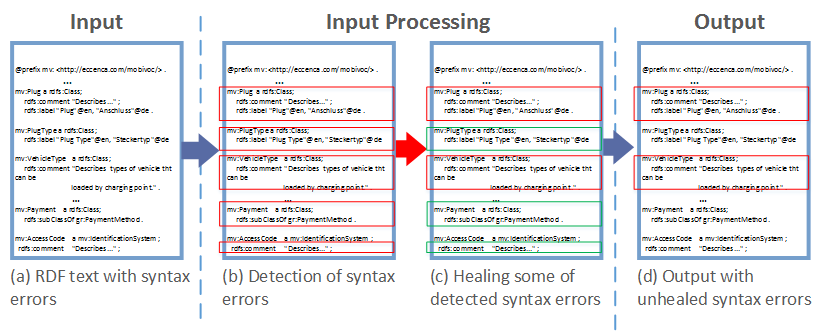
\includegraphics[width=13cm]{images/Approach.png}
		\caption{Overview of the Proposed Solution}
		\label{Fig:Approach}  
\end{figure}
\section{Representation in Pseudo-code}
To functionally represent the approach of this study, Algorithm \ref{alg:algorithm-main} was engineered. It is showing the abstract behaviour of the developed program where \textbf{syntaxRules} variable combines both correct syntax rules and incorrect ones. A \textbf{While loop} traverse till the end of the file or a single chunk if a large file was separated in a couple of chunks. The \textbf{tokensToBeMatched}  variable collected a sequence of followed tokens to be matched either with correct or incorrect syntax rules.

	\vspace{5mm} %5mm vertical space
Since our target is to find syntax errors,  s
	\vspace{5mm} %5mm vertical space

\begin{algorithm}[H] 
 \caption{Representation of the proposed solution  in pseudo-code}
 \label{alg:algorithm-main}
 \KwData{inputText, correctSyntaxRules, incorrectSyntaxRules, CorrectionIsSelected}
 \KwResult{foundSyntaxErrors and recoveredSyntaxErrors}

% S = subject(M)\;
foundSyntaxErrors = [ ];\\
recoveredSyntaxErrors = [ ];\\
$syntaxRules \leftarrow correctSyntaxRules + incorrectSyntaxRules;$\\
		\While{token in inputText \&\& $inputText \neq EOF$}{
tokenToBeMatched += token;\\
		\uIf{ syntaxRules contains tokensToBeMatched}{
		\uIf{ incorrectSyntaxRules contains tokensToBeMatched}{
		 foundSyntaxErrors.push(tokensToBeMatched);\\
		\uIf{ CorrectionIsSelected}{
		\uIf{ canErrorRecovered(tokensToBeMatched)}{
		  \uIf{recoverSyntaxError(tokensToBeMatched)}{
		  recoveredSyntaxErrors.push(tokensToBeMatched);\\
		  foundSyntaxErrors.pop(tokensToBeMatched);\\

		  }
		}
		}
		}
		 $tokensToBeMatched \leftarrow ""$  \\
		 $token \leftarrow ""$  	\\	
		}
}
return foundSyntaxErrors \&\& recoveredSyntaxErrors
\end{algorithm}


\section{Classification of RDF Syntax Errors}

\section{Real-World Use Cases}

 
